\documentclass[12pt]{article}
\usepackage[table]{xcolor}
\usepackage[shortlabels]{enumitem}
\usepackage{tabularx,xltabular}
\usepackage{graphicx}
\usepackage{hyperref}
\usepackage{verbatim}
\usepackage{geometry}
\usepackage{ulem}
\usepackage[official]{eurosym}
\usepackage{tikz}
\usetikzlibrary{arrows,backgrounds,calc,decorations.markings,patterns,3d,positioning,fit,angles, quotes}
\usepackage{pgfplots}
\pgfplotsset{compat = newest}
\usetikzlibrary{fit}
\newcommand\addvmargin[1]{
\usetikzlibrary{arrows}
\node[fit=(current bounding box),inner ysep=#1,inner xsep=0]{};}
\usepackage{cancel}
\usepackage{fontspec}
\usepackage{array}  
\geometry{a4paper, top=2cm, left=2cm, right=2cm, bottom=2cm, headsep=1cm}
\usepackage{tabu}
\usepackage{pst-node}
\usepackage{colortbl}
\usepackage{array}
\usepackage{german}
\setlength\parindent{0pt}
\newcolumntype{?}{!{\vrule width 1pt}}
\usepackage{makecell}
\renewcommand{\arraystretch}{2.5}
\usepackage{pbox}
\usepackage{amssymb}
\usepackage{amsmath}
\usepackage{booktabs}
\newcolumntype{L}[1]{>{\raggedright\let\newline\\\arraybackslash\hspace{0pt}}m{#1}}
\newcolumntype{C}[1]{>{\centering\let\newline\\\arraybackslash\hspace{0pt}}m{#1}}
\newcolumntype{R}[1]{>{\raggedleft\let\newline\\\arraybackslash\hspace{0pt}}m{#1}}
\begin{document}
\rightline{Datum: 12.12.2023}
\centerline{{\Large Tägliche Übungen}} 
\vspace{1cm}
\noindent \\


\begin{xltabular}{\textwidth}{|C{0.75cm}|X|}
\arrayrulecolor{black}\hline
a)&\pbox{15cm}{
Welche Fläche ist größer, grün oder Blau?\\
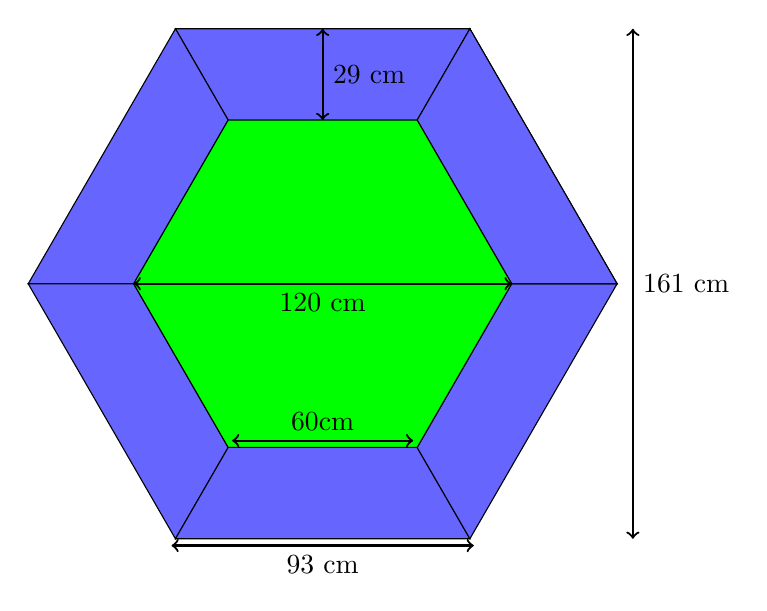
\begin{tikzpicture}
%Ich rechne mal sqrt(0.75) da hier ein gleichseitiges Dreieck vorliegt, bei dem man die Höhe berechnen muss.
%Dies geht mit dem Pythagoras, wobei der durch die Hälfte der Seite geht:
%               a²+b²=c² mit a=c/2 --> b²=c²-(c/2)²=c²-c²/4=3/4*c² --> b=c*sqrt(3/4)
%Flächenberechnung grün-blau in Python:
%R,h=50,25
%2*((2*R-R)*R*(0.75**0.5)/2)-6*((R+h*(0.75**0.5))-R)*h/2
  \pgfmathsetmacro{\hWert}{29}
  \pgfmathsetmacro{\RWert}{60}
  \pgfmathsetmacro{\dh}{\hWert/100*4}
  \pgfmathsetmacro{\R}{\RWert/100*4}
  \pgfmathsetmacro{\dR}{\dh/sqrt(0.75)}
  \pgfmathsetmacro{\hges}{(\R+\dR)*sqrt(0.75)}
  \pgfmathsetmacro{\h}{\hges-\dh}
%Schreibe ohne Komma
  \pgfmathtruncatemacro\gesamthoehe{2*(\RWert*sqrt(0.75)+\hWert)}
  \pgfmathtruncatemacro\aussenlaenge{\RWert+\hWert/sqrt(0.75)}
  \pgfmathtruncatemacro\innenlaenge{2*\RWert}
  \pgfmathtruncatemacro\innenhoehe{\RWert*sqrt(0.75)}
\foreach \rot in  {0,60,...,360}{
\draw[black,rotate=\rot,fill=blue!60] (\R,0) -- ++(\dR,0) -- ++(120:\R+\dR) -- ++(60:-\dR) -- cycle;
}
\draw[black,fill=green] (\R,0) -- ++(120:\R) -- ++(180:\R) -- ++(240:\R) -- ++(120:-\R) -- ++(0:\R) -- cycle ;
\draw[thick,<->] (-\R,0) --node[below] {\innenlaenge~cm} (\R,0);
\draw[thick,<->] (\R+\dR+0.2,\hges) --node[right] {\gesamthoehe~cm} (\R+\dR+0.2,-\hges) ;
\draw[thick,<->] (240:\R-0.1) --node[above] {\RWert cm}  (300:\R-0.1);
\draw[thick,<->] (240:\R+\dR+0.1) --node[below] {\aussenlaenge~cm}  (300:\R+\dR+0.1);
\draw[thick,<->] (0,\h) --node[right] {\hWert~cm} (0,\hges);
\end{tikzpicture}
}
\\\hline
b)&\pbox{15cm}{
Welche Fläche ist größer, grün oder Blau?\\
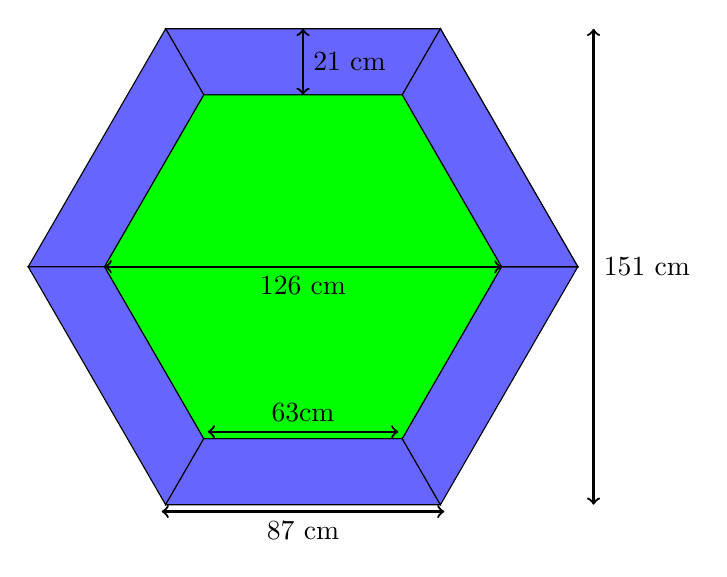
\begin{tikzpicture}
%Ich rechne mal sqrt(0.75) da hier ein gleichseitiges Dreieck vorliegt, bei dem man die Höhe berechnen muss.
%Dies geht mit dem Pythagoras, wobei der durch die Hälfte der Seite geht:
%               a²+b²=c² mit a=c/2 --> b²=c²-(c/2)²=c²-c²/4=3/4*c² --> b=c*sqrt(3/4)
%Flächenberechnung grün-blau in Python:
%R,h=50,25
%2*((2*R-R)*R*(0.75**0.5)/2)-6*((R+h*(0.75**0.5))-R)*h/2
  \pgfmathsetmacro{\hWert}{21}
  \pgfmathsetmacro{\RWert}{63}
  \pgfmathsetmacro{\dh}{\hWert/100*4}
  \pgfmathsetmacro{\R}{\RWert/100*4}
  \pgfmathsetmacro{\dR}{\dh/sqrt(0.75)}
  \pgfmathsetmacro{\hges}{(\R+\dR)*sqrt(0.75)}
  \pgfmathsetmacro{\h}{\hges-\dh}
%Schreibe ohne Komma
  \pgfmathtruncatemacro\gesamthoehe{2*(\RWert*sqrt(0.75)+\hWert)}
  \pgfmathtruncatemacro\aussenlaenge{\RWert+\hWert/sqrt(0.75)}
  \pgfmathtruncatemacro\innenlaenge{2*\RWert}
  \pgfmathtruncatemacro\innenhoehe{\RWert*sqrt(0.75)}
\foreach \rot in  {0,60,...,360}{
\draw[black,rotate=\rot,fill=blue!60] (\R,0) -- ++(\dR,0) -- ++(120:\R+\dR) -- ++(60:-\dR) -- cycle;
}
\draw[black,fill=green] (\R,0) -- ++(120:\R) -- ++(180:\R) -- ++(240:\R) -- ++(120:-\R) -- ++(0:\R) -- cycle ;
\draw[thick,<->] (-\R,0) --node[below] {\innenlaenge~cm} (\R,0);
\draw[thick,<->] (\R+\dR+0.2,\hges) --node[right] {\gesamthoehe~cm} (\R+\dR+0.2,-\hges) ;
\draw[thick,<->] (240:\R-0.1) --node[above] {\RWert cm}  (300:\R-0.1);
\draw[thick,<->] (240:\R+\dR+0.1) --node[below] {\aussenlaenge~cm}  (300:\R+\dR+0.1);
\draw[thick,<->] (0,\h) --node[right] {\hWert~cm} (0,\hges);
\end{tikzpicture}
}
\\\hline
c)&\pbox{15cm}{
Welche Fläche ist größer, grün oder Blau?\\
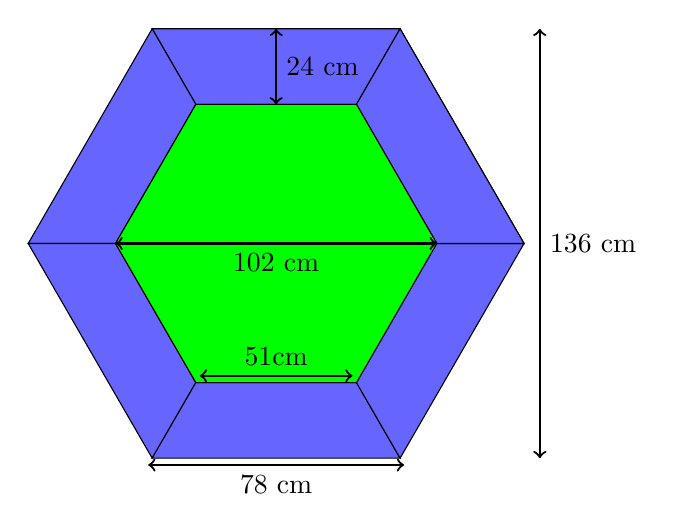
\begin{tikzpicture}
%Ich rechne mal sqrt(0.75) da hier ein gleichseitiges Dreieck vorliegt, bei dem man die Höhe berechnen muss.
%Dies geht mit dem Pythagoras, wobei der durch die Hälfte der Seite geht:
%               a²+b²=c² mit a=c/2 --> b²=c²-(c/2)²=c²-c²/4=3/4*c² --> b=c*sqrt(3/4)
%Flächenberechnung grün-blau in Python:
%R,h=50,25
%2*((2*R-R)*R*(0.75**0.5)/2)-6*((R+h*(0.75**0.5))-R)*h/2
  \pgfmathsetmacro{\hWert}{24}
  \pgfmathsetmacro{\RWert}{51}
  \pgfmathsetmacro{\dh}{\hWert/100*4}
  \pgfmathsetmacro{\R}{\RWert/100*4}
  \pgfmathsetmacro{\dR}{\dh/sqrt(0.75)}
  \pgfmathsetmacro{\hges}{(\R+\dR)*sqrt(0.75)}
  \pgfmathsetmacro{\h}{\hges-\dh}
%Schreibe ohne Komma
  \pgfmathtruncatemacro\gesamthoehe{2*(\RWert*sqrt(0.75)+\hWert)}
  \pgfmathtruncatemacro\aussenlaenge{\RWert+\hWert/sqrt(0.75)}
  \pgfmathtruncatemacro\innenlaenge{2*\RWert}
  \pgfmathtruncatemacro\innenhoehe{\RWert*sqrt(0.75)}
\foreach \rot in  {0,60,...,360}{
\draw[black,rotate=\rot,fill=blue!60] (\R,0) -- ++(\dR,0) -- ++(120:\R+\dR) -- ++(60:-\dR) -- cycle;
}
\draw[black,fill=green] (\R,0) -- ++(120:\R) -- ++(180:\R) -- ++(240:\R) -- ++(120:-\R) -- ++(0:\R) -- cycle ;
\draw[thick,<->] (-\R,0) --node[below] {\innenlaenge~cm} (\R,0);
\draw[thick,<->] (\R+\dR+0.2,\hges) --node[right] {\gesamthoehe~cm} (\R+\dR+0.2,-\hges) ;
\draw[thick,<->] (240:\R-0.1) --node[above] {\RWert cm}  (300:\R-0.1);
\draw[thick,<->] (240:\R+\dR+0.1) --node[below] {\aussenlaenge~cm}  (300:\R+\dR+0.1);
\draw[thick,<->] (0,\h) --node[right] {\hWert~cm} (0,\hges);
\end{tikzpicture}
}
\\\hline
d)&\pbox{15cm}{
Welche Fläche ist größer, grün oder Blau?\\
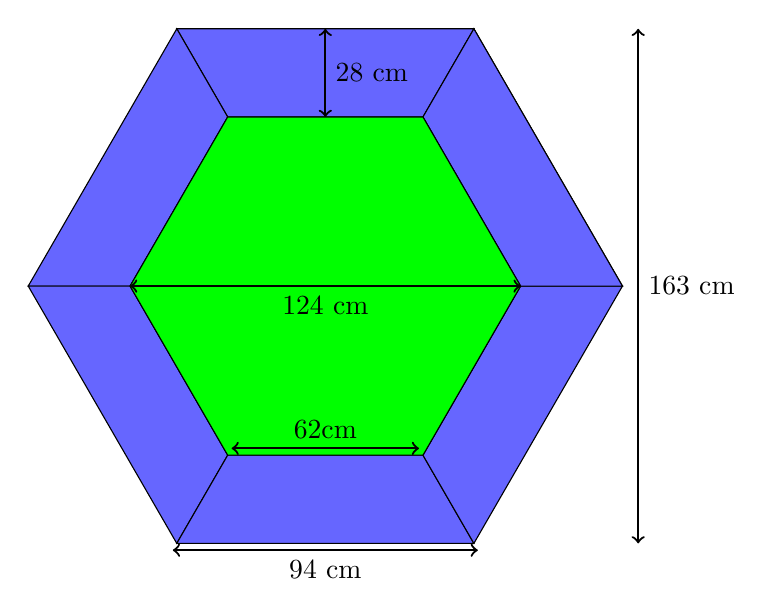
\begin{tikzpicture}
%Ich rechne mal sqrt(0.75) da hier ein gleichseitiges Dreieck vorliegt, bei dem man die Höhe berechnen muss.
%Dies geht mit dem Pythagoras, wobei der durch die Hälfte der Seite geht:
%               a²+b²=c² mit a=c/2 --> b²=c²-(c/2)²=c²-c²/4=3/4*c² --> b=c*sqrt(3/4)
%Flächenberechnung grün-blau in Python:
%R,h=50,25
%2*((2*R-R)*R*(0.75**0.5)/2)-6*((R+h*(0.75**0.5))-R)*h/2
  \pgfmathsetmacro{\hWert}{28}
  \pgfmathsetmacro{\RWert}{62}
  \pgfmathsetmacro{\dh}{\hWert/100*4}
  \pgfmathsetmacro{\R}{\RWert/100*4}
  \pgfmathsetmacro{\dR}{\dh/sqrt(0.75)}
  \pgfmathsetmacro{\hges}{(\R+\dR)*sqrt(0.75)}
  \pgfmathsetmacro{\h}{\hges-\dh}
%Schreibe ohne Komma
  \pgfmathtruncatemacro\gesamthoehe{2*(\RWert*sqrt(0.75)+\hWert)}
  \pgfmathtruncatemacro\aussenlaenge{\RWert+\hWert/sqrt(0.75)}
  \pgfmathtruncatemacro\innenlaenge{2*\RWert}
  \pgfmathtruncatemacro\innenhoehe{\RWert*sqrt(0.75)}
\foreach \rot in  {0,60,...,360}{
\draw[black,rotate=\rot,fill=blue!60] (\R,0) -- ++(\dR,0) -- ++(120:\R+\dR) -- ++(60:-\dR) -- cycle;
}
\draw[black,fill=green] (\R,0) -- ++(120:\R) -- ++(180:\R) -- ++(240:\R) -- ++(120:-\R) -- ++(0:\R) -- cycle ;
\draw[thick,<->] (-\R,0) --node[below] {\innenlaenge~cm} (\R,0);
\draw[thick,<->] (\R+\dR+0.2,\hges) --node[right] {\gesamthoehe~cm} (\R+\dR+0.2,-\hges) ;
\draw[thick,<->] (240:\R-0.1) --node[above] {\RWert cm}  (300:\R-0.1);
\draw[thick,<->] (240:\R+\dR+0.1) --node[below] {\aussenlaenge~cm}  (300:\R+\dR+0.1);
\draw[thick,<->] (0,\h) --node[right] {\hWert~cm} (0,\hges);
\end{tikzpicture}
}
\\\hline
e)&\pbox{15cm}{
Welche Fläche ist größer, grün oder Blau?\\
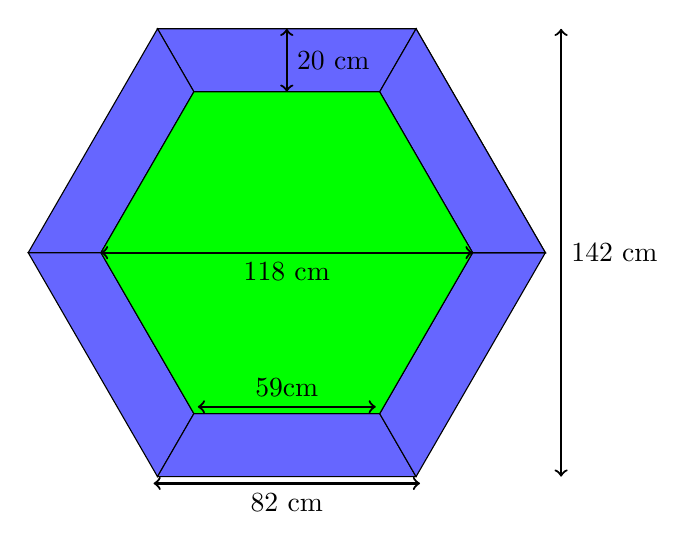
\begin{tikzpicture}
%Ich rechne mal sqrt(0.75) da hier ein gleichseitiges Dreieck vorliegt, bei dem man die Höhe berechnen muss.
%Dies geht mit dem Pythagoras, wobei der durch die Hälfte der Seite geht:
%               a²+b²=c² mit a=c/2 --> b²=c²-(c/2)²=c²-c²/4=3/4*c² --> b=c*sqrt(3/4)
%Flächenberechnung grün-blau in Python:
%R,h=50,25
%2*((2*R-R)*R*(0.75**0.5)/2)-6*((R+h*(0.75**0.5))-R)*h/2
  \pgfmathsetmacro{\hWert}{20}
  \pgfmathsetmacro{\RWert}{59}
  \pgfmathsetmacro{\dh}{\hWert/100*4}
  \pgfmathsetmacro{\R}{\RWert/100*4}
  \pgfmathsetmacro{\dR}{\dh/sqrt(0.75)}
  \pgfmathsetmacro{\hges}{(\R+\dR)*sqrt(0.75)}
  \pgfmathsetmacro{\h}{\hges-\dh}
%Schreibe ohne Komma
  \pgfmathtruncatemacro\gesamthoehe{2*(\RWert*sqrt(0.75)+\hWert)}
  \pgfmathtruncatemacro\aussenlaenge{\RWert+\hWert/sqrt(0.75)}
  \pgfmathtruncatemacro\innenlaenge{2*\RWert}
  \pgfmathtruncatemacro\innenhoehe{\RWert*sqrt(0.75)}
\foreach \rot in  {0,60,...,360}{
\draw[black,rotate=\rot,fill=blue!60] (\R,0) -- ++(\dR,0) -- ++(120:\R+\dR) -- ++(60:-\dR) -- cycle;
}
\draw[black,fill=green] (\R,0) -- ++(120:\R) -- ++(180:\R) -- ++(240:\R) -- ++(120:-\R) -- ++(0:\R) -- cycle ;
\draw[thick,<->] (-\R,0) --node[below] {\innenlaenge~cm} (\R,0);
\draw[thick,<->] (\R+\dR+0.2,\hges) --node[right] {\gesamthoehe~cm} (\R+\dR+0.2,-\hges) ;
\draw[thick,<->] (240:\R-0.1) --node[above] {\RWert cm}  (300:\R-0.1);
\draw[thick,<->] (240:\R+\dR+0.1) --node[below] {\aussenlaenge~cm}  (300:\R+\dR+0.1);
\draw[thick,<->] (0,\h) --node[right] {\hWert~cm} (0,\hges);
\end{tikzpicture}
}
\\\hline
f)&\pbox{15cm}{
Welche Fläche ist größer, grün oder Blau?\\
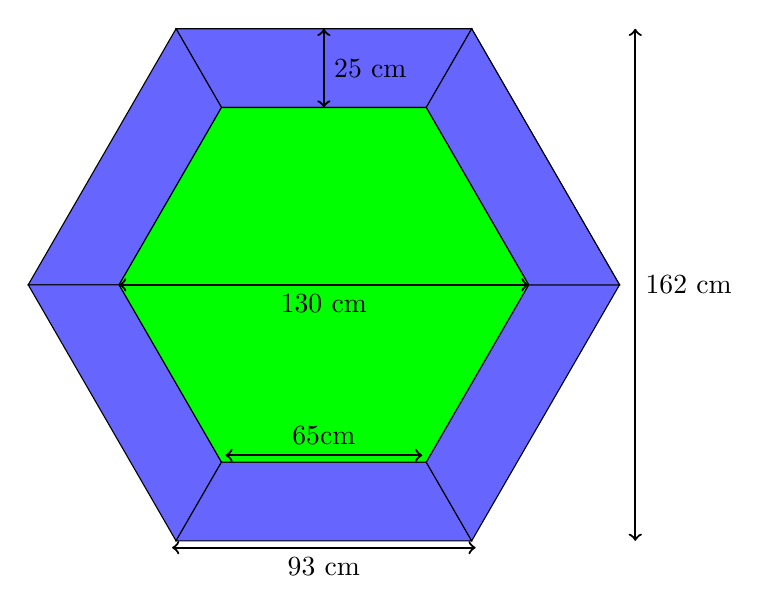
\begin{tikzpicture}
%Ich rechne mal sqrt(0.75) da hier ein gleichseitiges Dreieck vorliegt, bei dem man die Höhe berechnen muss.
%Dies geht mit dem Pythagoras, wobei der durch die Hälfte der Seite geht:
%               a²+b²=c² mit a=c/2 --> b²=c²-(c/2)²=c²-c²/4=3/4*c² --> b=c*sqrt(3/4)
%Flächenberechnung grün-blau in Python:
%R,h=50,25
%2*((2*R-R)*R*(0.75**0.5)/2)-6*((R+h*(0.75**0.5))-R)*h/2
  \pgfmathsetmacro{\hWert}{25}
  \pgfmathsetmacro{\RWert}{65}
  \pgfmathsetmacro{\dh}{\hWert/100*4}
  \pgfmathsetmacro{\R}{\RWert/100*4}
  \pgfmathsetmacro{\dR}{\dh/sqrt(0.75)}
  \pgfmathsetmacro{\hges}{(\R+\dR)*sqrt(0.75)}
  \pgfmathsetmacro{\h}{\hges-\dh}
%Schreibe ohne Komma
  \pgfmathtruncatemacro\gesamthoehe{2*(\RWert*sqrt(0.75)+\hWert)}
  \pgfmathtruncatemacro\aussenlaenge{\RWert+\hWert/sqrt(0.75)}
  \pgfmathtruncatemacro\innenlaenge{2*\RWert}
  \pgfmathtruncatemacro\innenhoehe{\RWert*sqrt(0.75)}
\foreach \rot in  {0,60,...,360}{
\draw[black,rotate=\rot,fill=blue!60] (\R,0) -- ++(\dR,0) -- ++(120:\R+\dR) -- ++(60:-\dR) -- cycle;
}
\draw[black,fill=green] (\R,0) -- ++(120:\R) -- ++(180:\R) -- ++(240:\R) -- ++(120:-\R) -- ++(0:\R) -- cycle ;
\draw[thick,<->] (-\R,0) --node[below] {\innenlaenge~cm} (\R,0);
\draw[thick,<->] (\R+\dR+0.2,\hges) --node[right] {\gesamthoehe~cm} (\R+\dR+0.2,-\hges) ;
\draw[thick,<->] (240:\R-0.1) --node[above] {\RWert cm}  (300:\R-0.1);
\draw[thick,<->] (240:\R+\dR+0.1) --node[below] {\aussenlaenge~cm}  (300:\R+\dR+0.1);
\draw[thick,<->] (0,\h) --node[right] {\hWert~cm} (0,\hges);
\end{tikzpicture}
}
\\\hline
g)&\pbox{15cm}{
Welche Fläche ist größer, grün oder Blau?\\
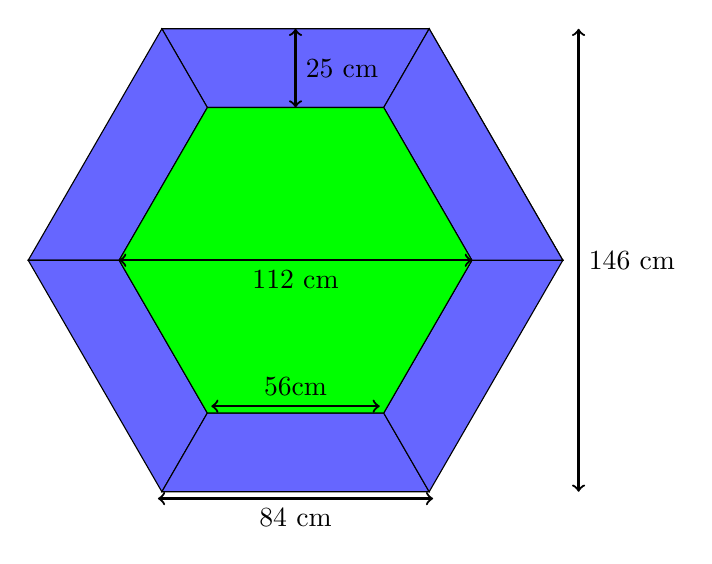
\begin{tikzpicture}
%Ich rechne mal sqrt(0.75) da hier ein gleichseitiges Dreieck vorliegt, bei dem man die Höhe berechnen muss.
%Dies geht mit dem Pythagoras, wobei der durch die Hälfte der Seite geht:
%               a²+b²=c² mit a=c/2 --> b²=c²-(c/2)²=c²-c²/4=3/4*c² --> b=c*sqrt(3/4)
%Flächenberechnung grün-blau in Python:
%R,h=50,25
%2*((2*R-R)*R*(0.75**0.5)/2)-6*((R+h*(0.75**0.5))-R)*h/2
  \pgfmathsetmacro{\hWert}{25}
  \pgfmathsetmacro{\RWert}{56}
  \pgfmathsetmacro{\dh}{\hWert/100*4}
  \pgfmathsetmacro{\R}{\RWert/100*4}
  \pgfmathsetmacro{\dR}{\dh/sqrt(0.75)}
  \pgfmathsetmacro{\hges}{(\R+\dR)*sqrt(0.75)}
  \pgfmathsetmacro{\h}{\hges-\dh}
%Schreibe ohne Komma
  \pgfmathtruncatemacro\gesamthoehe{2*(\RWert*sqrt(0.75)+\hWert)}
  \pgfmathtruncatemacro\aussenlaenge{\RWert+\hWert/sqrt(0.75)}
  \pgfmathtruncatemacro\innenlaenge{2*\RWert}
  \pgfmathtruncatemacro\innenhoehe{\RWert*sqrt(0.75)}
\foreach \rot in  {0,60,...,360}{
\draw[black,rotate=\rot,fill=blue!60] (\R,0) -- ++(\dR,0) -- ++(120:\R+\dR) -- ++(60:-\dR) -- cycle;
}
\draw[black,fill=green] (\R,0) -- ++(120:\R) -- ++(180:\R) -- ++(240:\R) -- ++(120:-\R) -- ++(0:\R) -- cycle ;
\draw[thick,<->] (-\R,0) --node[below] {\innenlaenge~cm} (\R,0);
\draw[thick,<->] (\R+\dR+0.2,\hges) --node[right] {\gesamthoehe~cm} (\R+\dR+0.2,-\hges) ;
\draw[thick,<->] (240:\R-0.1) --node[above] {\RWert cm}  (300:\R-0.1);
\draw[thick,<->] (240:\R+\dR+0.1) --node[below] {\aussenlaenge~cm}  (300:\R+\dR+0.1);
\draw[thick,<->] (0,\h) --node[right] {\hWert~cm} (0,\hges);
\end{tikzpicture}
}
\\\hline
h)&\pbox{15cm}{
Welche Fläche ist größer, grün oder Blau?\\
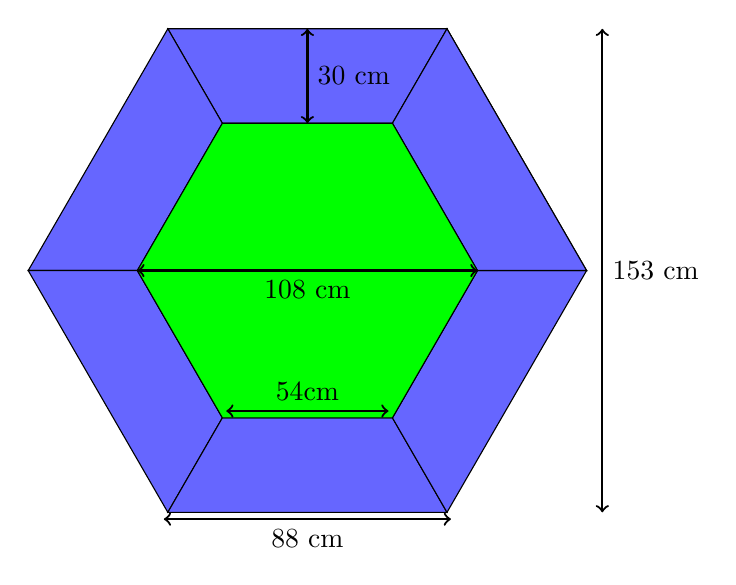
\begin{tikzpicture}
%Ich rechne mal sqrt(0.75) da hier ein gleichseitiges Dreieck vorliegt, bei dem man die Höhe berechnen muss.
%Dies geht mit dem Pythagoras, wobei der durch die Hälfte der Seite geht:
%               a²+b²=c² mit a=c/2 --> b²=c²-(c/2)²=c²-c²/4=3/4*c² --> b=c*sqrt(3/4)
%Flächenberechnung grün-blau in Python:
%R,h=50,25
%2*((2*R-R)*R*(0.75**0.5)/2)-6*((R+h*(0.75**0.5))-R)*h/2
  \pgfmathsetmacro{\hWert}{30}
  \pgfmathsetmacro{\RWert}{54}
  \pgfmathsetmacro{\dh}{\hWert/100*4}
  \pgfmathsetmacro{\R}{\RWert/100*4}
  \pgfmathsetmacro{\dR}{\dh/sqrt(0.75)}
  \pgfmathsetmacro{\hges}{(\R+\dR)*sqrt(0.75)}
  \pgfmathsetmacro{\h}{\hges-\dh}
%Schreibe ohne Komma
  \pgfmathtruncatemacro\gesamthoehe{2*(\RWert*sqrt(0.75)+\hWert)}
  \pgfmathtruncatemacro\aussenlaenge{\RWert+\hWert/sqrt(0.75)}
  \pgfmathtruncatemacro\innenlaenge{2*\RWert}
  \pgfmathtruncatemacro\innenhoehe{\RWert*sqrt(0.75)}
\foreach \rot in  {0,60,...,360}{
\draw[black,rotate=\rot,fill=blue!60] (\R,0) -- ++(\dR,0) -- ++(120:\R+\dR) -- ++(60:-\dR) -- cycle;
}
\draw[black,fill=green] (\R,0) -- ++(120:\R) -- ++(180:\R) -- ++(240:\R) -- ++(120:-\R) -- ++(0:\R) -- cycle ;
\draw[thick,<->] (-\R,0) --node[below] {\innenlaenge~cm} (\R,0);
\draw[thick,<->] (\R+\dR+0.2,\hges) --node[right] {\gesamthoehe~cm} (\R+\dR+0.2,-\hges) ;
\draw[thick,<->] (240:\R-0.1) --node[above] {\RWert cm}  (300:\R-0.1);
\draw[thick,<->] (240:\R+\dR+0.1) --node[below] {\aussenlaenge~cm}  (300:\R+\dR+0.1);
\draw[thick,<->] (0,\h) --node[right] {\hWert~cm} (0,\hges);
\end{tikzpicture}
}
\\\hline
\end{xltabular}
\vspace{0.5cm}
\newpage
\rightline{Datum: 12.12.2023}
\centerline{{\large Lösungen Tägliche Übungen}} 
\vspace{0.5cm}

\begin{xltabular}{\textwidth}{|C{0.75cm}|X|}
\arrayrulecolor{black}\hline
a)&\pbox{7cm}{
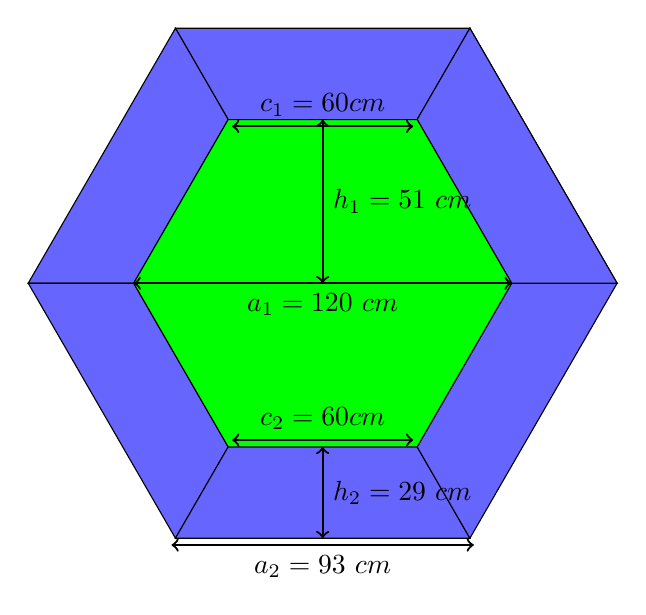
\begin{tikzpicture}
%Ich rechne mal sqrt(0.75) da hier ein gleichseitiges Dreieck vorliegt, bei dem man die Höhe berechnen muss.
%Dies geht mit dem Pythagoras, wobei der durch die Hälfte der Seite geht:
%               a²+b²=c² mit a=c/2 --> b²=c²-(c/2)²=c²-c²/4=3/4*c² --> b=c*sqrt(3/4)
%Flächenberechnung grün-blau in Python:
%R,h=50,25
%2*((2*R-R)*R*(0.75**0.5)/2)-6*((R+h*(0.75**0.5))-R)*h/2
  \pgfmathsetmacro{\hWert}{29}
  \pgfmathsetmacro{\RWert}{60}
  \pgfmathsetmacro{\dh}{\hWert/100*4}
  \pgfmathsetmacro{\R}{\RWert/100*4}
  \pgfmathsetmacro{\dR}{\dh/sqrt(0.75)}
  \pgfmathsetmacro{\hges}{(\R+\dR)*sqrt(0.75)}
  \pgfmathsetmacro{\h}{\hges-\dh}
%Schreibe ohne Komma
  \pgfmathtruncatemacro\gesamthoehe{2*(\RWert*sqrt(0.75)+\hWert)}
  \pgfmathtruncatemacro\aussenlaenge{\RWert+\hWert/sqrt(0.75)}
  \pgfmathtruncatemacro\innenlaenge{2*\RWert}
  \pgfmathtruncatemacro\innenhoehe{\RWert*sqrt(0.75)}
\foreach \rot in  {0,60,...,360}{
\draw[black,rotate=\rot,fill=blue!60] (\R,0) -- ++(\dR,0) -- ++(120:\R+\dR) -- ++(60:-\dR) -- cycle;
}
\draw[black,fill=green] (\R,0) -- ++(120:\R) -- ++(180:\R) -- ++(240:\R) -- ++(120:-\R) -- ++(0:\R) -- cycle ;
\draw[thick,<->] (-\R,0) --node[below] {$a_1=\innenlaenge~cm$} (\R,0);
\draw[thick,<->] (240:\R+\dR+0.1) --node[below] {$a_2=\aussenlaenge~cm$}  (300:\R+\dR+0.1);
\draw[thick,<->] (0,-\h) --node[right] {$h_2=\hWert~cm$} (0,-\hges);
\draw[thick,<->] (0,0) --node[right] {$h_1=\innenhoehe~cm$} (0,\h);
\draw[thick,<->] (240:\R-0.1) --node[above] {$c_2=\RWert cm$}  (300:\R-0.1);
\draw[thick,<->] (60:\R-0.1) --node[above] {$c_1=\RWert cm$}  (120:\R-0.1);
\end{tikzpicture}
$\begin{aligned}
geg.: a_1 &=120~cm& & \\
  c_1 &=60~cm& & \\
  h_1 &=160:2-29=51~cm& & \\
  a_2 &=93~cm& & \\
  c_2 &=60~cm& & \\
  h_2 &=29~cm & \\
ges.: A_{Gruen} &=?~cm^2& & \\
 A_{Blau} &=?~cm^2& & \\
& & & \\
A_{Gruen}&= 2\cdot (\frac12(a_1+c_1)\cdot h_1) & & \\
&= 2\cdot (\frac12(120+60)\cdot 51) & & \\
\makebox[0pt][l]{\uuline{\phantom{$A_{Gruen}=9.180~cm^2   \\$} } }
A_{Gruen}&=9.180~cm^2 & & \\
& & & \\
A_{blau}&= 6\cdot (\frac12(a_2+c_2)\cdot h_2) & & \\
&= 6\cdot (\frac12(93+60)\cdot 29) & & \\
\makebox[0pt][l]{\uuline{\phantom{$A_{blau}=13.353,31~cm^2   \\$} } }
A_{blau}&=13.353,31~cm^2 & & \\
\end{aligned}$
Die blaue Fläche ist größer.
}
\\\hline
b)&\pbox{7cm}{
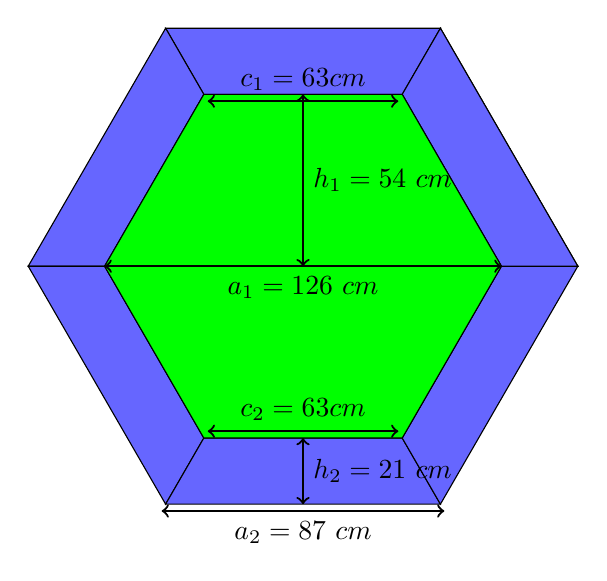
\begin{tikzpicture}
%Ich rechne mal sqrt(0.75) da hier ein gleichseitiges Dreieck vorliegt, bei dem man die Höhe berechnen muss.
%Dies geht mit dem Pythagoras, wobei der durch die Hälfte der Seite geht:
%               a²+b²=c² mit a=c/2 --> b²=c²-(c/2)²=c²-c²/4=3/4*c² --> b=c*sqrt(3/4)
%Flächenberechnung grün-blau in Python:
%R,h=50,25
%2*((2*R-R)*R*(0.75**0.5)/2)-6*((R+h*(0.75**0.5))-R)*h/2
  \pgfmathsetmacro{\hWert}{21}
  \pgfmathsetmacro{\RWert}{63}
  \pgfmathsetmacro{\dh}{\hWert/100*4}
  \pgfmathsetmacro{\R}{\RWert/100*4}
  \pgfmathsetmacro{\dR}{\dh/sqrt(0.75)}
  \pgfmathsetmacro{\hges}{(\R+\dR)*sqrt(0.75)}
  \pgfmathsetmacro{\h}{\hges-\dh}
%Schreibe ohne Komma
  \pgfmathtruncatemacro\gesamthoehe{2*(\RWert*sqrt(0.75)+\hWert)}
  \pgfmathtruncatemacro\aussenlaenge{\RWert+\hWert/sqrt(0.75)}
  \pgfmathtruncatemacro\innenlaenge{2*\RWert}
  \pgfmathtruncatemacro\innenhoehe{\RWert*sqrt(0.75)}
\foreach \rot in  {0,60,...,360}{
\draw[black,rotate=\rot,fill=blue!60] (\R,0) -- ++(\dR,0) -- ++(120:\R+\dR) -- ++(60:-\dR) -- cycle;
}
\draw[black,fill=green] (\R,0) -- ++(120:\R) -- ++(180:\R) -- ++(240:\R) -- ++(120:-\R) -- ++(0:\R) -- cycle ;
\draw[thick,<->] (-\R,0) --node[below] {$a_1=\innenlaenge~cm$} (\R,0);
\draw[thick,<->] (240:\R+\dR+0.1) --node[below] {$a_2=\aussenlaenge~cm$}  (300:\R+\dR+0.1);
\draw[thick,<->] (0,-\h) --node[right] {$h_2=\hWert~cm$} (0,-\hges);
\draw[thick,<->] (0,0) --node[right] {$h_1=\innenhoehe~cm$} (0,\h);
\draw[thick,<->] (240:\R-0.1) --node[above] {$c_2=\RWert cm$}  (300:\R-0.1);
\draw[thick,<->] (60:\R-0.1) --node[above] {$c_1=\RWert cm$}  (120:\R-0.1);
\end{tikzpicture}
$\begin{aligned}
geg.: a_1 &=126~cm& & \\
  c_1 &=63~cm& & \\
  h_1 &=150:2-21=54~cm& & \\
  a_2 &=87~cm& & \\
  c_2 &=63~cm& & \\
  h_2 &=21~cm & \\
ges.: A_{Gruen} &=?~cm^2& & \\
 A_{Blau} &=?~cm^2& & \\
& & & \\
A_{Gruen}&= 2\cdot (\frac12(a_1+c_1)\cdot h_1) & & \\
&= 2\cdot (\frac12(126+63)\cdot 54) & & \\
\makebox[0pt][l]{\uuline{\phantom{$A_{Gruen}=10.206~cm^2   \\$} } }
A_{Gruen}&=10.206~cm^2 & & \\
& & & \\
A_{blau}&= 6\cdot (\frac12(a_2+c_2)\cdot h_2) & & \\
&= 6\cdot (\frac12(87+63)\cdot 21) & & \\
\makebox[0pt][l]{\uuline{\phantom{$A_{blau}=9.465,67~cm^2   \\$} } }
A_{blau}&=9.465,67~cm^2 & & \\
\end{aligned}$
Die grüne Fläche ist größer.
}
\\\hline
c)&\pbox{7cm}{
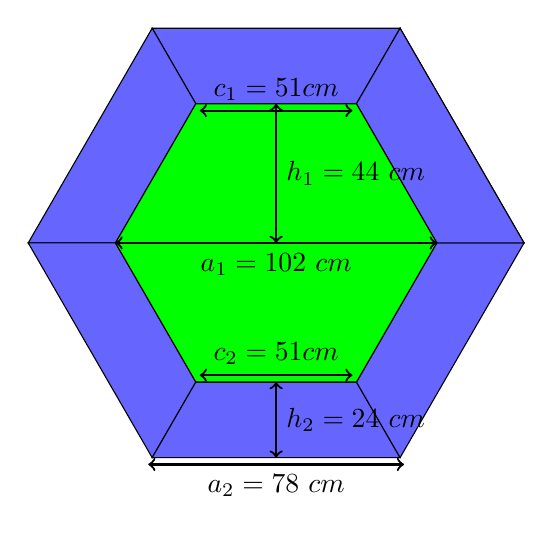
\begin{tikzpicture}
%Ich rechne mal sqrt(0.75) da hier ein gleichseitiges Dreieck vorliegt, bei dem man die Höhe berechnen muss.
%Dies geht mit dem Pythagoras, wobei der durch die Hälfte der Seite geht:
%               a²+b²=c² mit a=c/2 --> b²=c²-(c/2)²=c²-c²/4=3/4*c² --> b=c*sqrt(3/4)
%Flächenberechnung grün-blau in Python:
%R,h=50,25
%2*((2*R-R)*R*(0.75**0.5)/2)-6*((R+h*(0.75**0.5))-R)*h/2
  \pgfmathsetmacro{\hWert}{24}
  \pgfmathsetmacro{\RWert}{51}
  \pgfmathsetmacro{\dh}{\hWert/100*4}
  \pgfmathsetmacro{\R}{\RWert/100*4}
  \pgfmathsetmacro{\dR}{\dh/sqrt(0.75)}
  \pgfmathsetmacro{\hges}{(\R+\dR)*sqrt(0.75)}
  \pgfmathsetmacro{\h}{\hges-\dh}
%Schreibe ohne Komma
  \pgfmathtruncatemacro\gesamthoehe{2*(\RWert*sqrt(0.75)+\hWert)}
  \pgfmathtruncatemacro\aussenlaenge{\RWert+\hWert/sqrt(0.75)}
  \pgfmathtruncatemacro\innenlaenge{2*\RWert}
  \pgfmathtruncatemacro\innenhoehe{\RWert*sqrt(0.75)}
\foreach \rot in  {0,60,...,360}{
\draw[black,rotate=\rot,fill=blue!60] (\R,0) -- ++(\dR,0) -- ++(120:\R+\dR) -- ++(60:-\dR) -- cycle;
}
\draw[black,fill=green] (\R,0) -- ++(120:\R) -- ++(180:\R) -- ++(240:\R) -- ++(120:-\R) -- ++(0:\R) -- cycle ;
\draw[thick,<->] (-\R,0) --node[below] {$a_1=\innenlaenge~cm$} (\R,0);
\draw[thick,<->] (240:\R+\dR+0.1) --node[below] {$a_2=\aussenlaenge~cm$}  (300:\R+\dR+0.1);
\draw[thick,<->] (0,-\h) --node[right] {$h_2=\hWert~cm$} (0,-\hges);
\draw[thick,<->] (0,0) --node[right] {$h_1=\innenhoehe~cm$} (0,\h);
\draw[thick,<->] (240:\R-0.1) --node[above] {$c_2=\RWert cm$}  (300:\R-0.1);
\draw[thick,<->] (60:\R-0.1) --node[above] {$c_1=\RWert cm$}  (120:\R-0.1);
\end{tikzpicture}
$\begin{aligned}
geg.: a_1 &=102~cm& & \\
  c_1 &=51~cm& & \\
  h_1 &=136:2-24=44~cm& & \\
  a_2 &=78~cm& & \\
  c_2 &=51~cm& & \\
  h_2 &=24~cm & \\
ges.: A_{Gruen} &=?~cm^2& & \\
 A_{Blau} &=?~cm^2& & \\
& & & \\
A_{Gruen}&= 2\cdot (\frac12(a_1+c_1)\cdot h_1) & & \\
&= 2\cdot (\frac12(102+51)\cdot 44) & & \\
\makebox[0pt][l]{\uuline{\phantom{$A_{Gruen}=6.732~cm^2   \\$} } }
A_{Gruen}&=6.732~cm^2 & & \\
& & & \\
A_{blau}&= 6\cdot (\frac12(a_2+c_2)\cdot h_2) & & \\
&= 6\cdot (\frac12(78+51)\cdot 24) & & \\
\makebox[0pt][l]{\uuline{\phantom{$A_{blau}=9.339,32~cm^2   \\$} } }
A_{blau}&=9.339,32~cm^2 & & \\
\end{aligned}$
Die blaue Fläche ist größer.
}
\\\hline
d)&\pbox{7cm}{
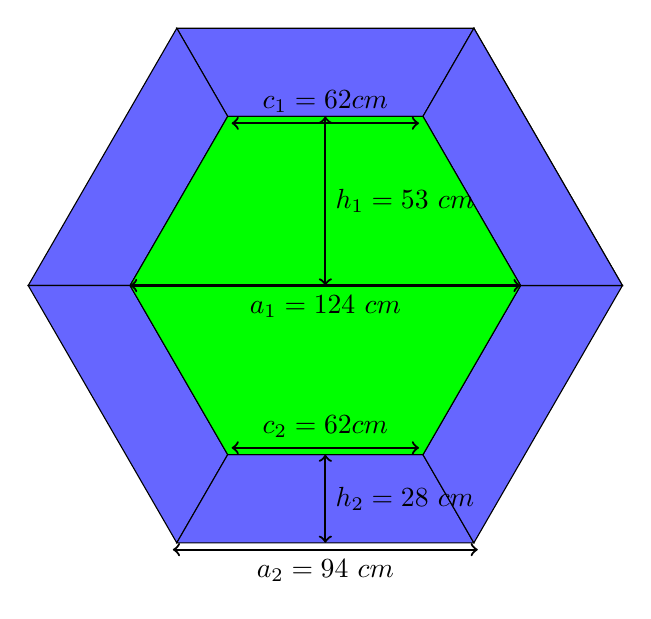
\begin{tikzpicture}
%Ich rechne mal sqrt(0.75) da hier ein gleichseitiges Dreieck vorliegt, bei dem man die Höhe berechnen muss.
%Dies geht mit dem Pythagoras, wobei der durch die Hälfte der Seite geht:
%               a²+b²=c² mit a=c/2 --> b²=c²-(c/2)²=c²-c²/4=3/4*c² --> b=c*sqrt(3/4)
%Flächenberechnung grün-blau in Python:
%R,h=50,25
%2*((2*R-R)*R*(0.75**0.5)/2)-6*((R+h*(0.75**0.5))-R)*h/2
  \pgfmathsetmacro{\hWert}{28}
  \pgfmathsetmacro{\RWert}{62}
  \pgfmathsetmacro{\dh}{\hWert/100*4}
  \pgfmathsetmacro{\R}{\RWert/100*4}
  \pgfmathsetmacro{\dR}{\dh/sqrt(0.75)}
  \pgfmathsetmacro{\hges}{(\R+\dR)*sqrt(0.75)}
  \pgfmathsetmacro{\h}{\hges-\dh}
%Schreibe ohne Komma
  \pgfmathtruncatemacro\gesamthoehe{2*(\RWert*sqrt(0.75)+\hWert)}
  \pgfmathtruncatemacro\aussenlaenge{\RWert+\hWert/sqrt(0.75)}
  \pgfmathtruncatemacro\innenlaenge{2*\RWert}
  \pgfmathtruncatemacro\innenhoehe{\RWert*sqrt(0.75)}
\foreach \rot in  {0,60,...,360}{
\draw[black,rotate=\rot,fill=blue!60] (\R,0) -- ++(\dR,0) -- ++(120:\R+\dR) -- ++(60:-\dR) -- cycle;
}
\draw[black,fill=green] (\R,0) -- ++(120:\R) -- ++(180:\R) -- ++(240:\R) -- ++(120:-\R) -- ++(0:\R) -- cycle ;
\draw[thick,<->] (-\R,0) --node[below] {$a_1=\innenlaenge~cm$} (\R,0);
\draw[thick,<->] (240:\R+\dR+0.1) --node[below] {$a_2=\aussenlaenge~cm$}  (300:\R+\dR+0.1);
\draw[thick,<->] (0,-\h) --node[right] {$h_2=\hWert~cm$} (0,-\hges);
\draw[thick,<->] (0,0) --node[right] {$h_1=\innenhoehe~cm$} (0,\h);
\draw[thick,<->] (240:\R-0.1) --node[above] {$c_2=\RWert cm$}  (300:\R-0.1);
\draw[thick,<->] (60:\R-0.1) --node[above] {$c_1=\RWert cm$}  (120:\R-0.1);
\end{tikzpicture}
$\begin{aligned}
geg.: a_1 &=124~cm& & \\
  c_1 &=62~cm& & \\
  h_1 &=162:2-28=53~cm& & \\
  a_2 &=94~cm& & \\
  c_2 &=62~cm& & \\
  h_2 &=28~cm & \\
ges.: A_{Gruen} &=?~cm^2& & \\
 A_{Blau} &=?~cm^2& & \\
& & & \\
A_{Gruen}&= 2\cdot (\frac12(a_1+c_1)\cdot h_1) & & \\
&= 2\cdot (\frac12(124+62)\cdot 53) & & \\
\makebox[0pt][l]{\uuline{\phantom{$A_{Gruen}=9.858~cm^2   \\$} } }
A_{Gruen}&=9.858~cm^2 & & \\
& & & \\
A_{blau}&= 6\cdot (\frac12(a_2+c_2)\cdot h_2) & & \\
&= 6\cdot (\frac12(94+62)\cdot 28) & & \\
\makebox[0pt][l]{\uuline{\phantom{$A_{blau}=13.131,86~cm^2   \\$} } }
A_{blau}&=13.131,86~cm^2 & & \\
\end{aligned}$
Die blaue Fläche ist größer.
}
\\\hline
e)&\pbox{7cm}{
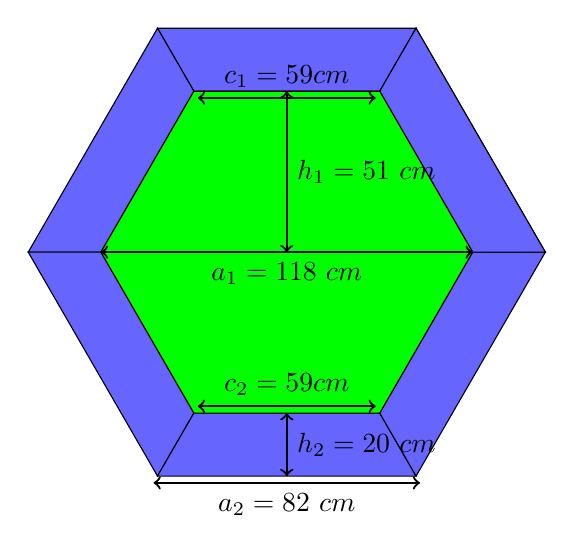
\begin{tikzpicture}
%Ich rechne mal sqrt(0.75) da hier ein gleichseitiges Dreieck vorliegt, bei dem man die Höhe berechnen muss.
%Dies geht mit dem Pythagoras, wobei der durch die Hälfte der Seite geht:
%               a²+b²=c² mit a=c/2 --> b²=c²-(c/2)²=c²-c²/4=3/4*c² --> b=c*sqrt(3/4)
%Flächenberechnung grün-blau in Python:
%R,h=50,25
%2*((2*R-R)*R*(0.75**0.5)/2)-6*((R+h*(0.75**0.5))-R)*h/2
  \pgfmathsetmacro{\hWert}{20}
  \pgfmathsetmacro{\RWert}{59}
  \pgfmathsetmacro{\dh}{\hWert/100*4}
  \pgfmathsetmacro{\R}{\RWert/100*4}
  \pgfmathsetmacro{\dR}{\dh/sqrt(0.75)}
  \pgfmathsetmacro{\hges}{(\R+\dR)*sqrt(0.75)}
  \pgfmathsetmacro{\h}{\hges-\dh}
%Schreibe ohne Komma
  \pgfmathtruncatemacro\gesamthoehe{2*(\RWert*sqrt(0.75)+\hWert)}
  \pgfmathtruncatemacro\aussenlaenge{\RWert+\hWert/sqrt(0.75)}
  \pgfmathtruncatemacro\innenlaenge{2*\RWert}
  \pgfmathtruncatemacro\innenhoehe{\RWert*sqrt(0.75)}
\foreach \rot in  {0,60,...,360}{
\draw[black,rotate=\rot,fill=blue!60] (\R,0) -- ++(\dR,0) -- ++(120:\R+\dR) -- ++(60:-\dR) -- cycle;
}
\draw[black,fill=green] (\R,0) -- ++(120:\R) -- ++(180:\R) -- ++(240:\R) -- ++(120:-\R) -- ++(0:\R) -- cycle ;
\draw[thick,<->] (-\R,0) --node[below] {$a_1=\innenlaenge~cm$} (\R,0);
\draw[thick,<->] (240:\R+\dR+0.1) --node[below] {$a_2=\aussenlaenge~cm$}  (300:\R+\dR+0.1);
\draw[thick,<->] (0,-\h) --node[right] {$h_2=\hWert~cm$} (0,-\hges);
\draw[thick,<->] (0,0) --node[right] {$h_1=\innenhoehe~cm$} (0,\h);
\draw[thick,<->] (240:\R-0.1) --node[above] {$c_2=\RWert cm$}  (300:\R-0.1);
\draw[thick,<->] (60:\R-0.1) --node[above] {$c_1=\RWert cm$}  (120:\R-0.1);
\end{tikzpicture}
$\begin{aligned}
geg.: a_1 &=118~cm& & \\
  c_1 &=59~cm& & \\
  h_1 &=142:2-20=51~cm& & \\
  a_2 &=82~cm& & \\
  c_2 &=59~cm& & \\
  h_2 &=20~cm & \\
ges.: A_{Gruen} &=?~cm^2& & \\
 A_{Blau} &=?~cm^2& & \\
& & & \\
A_{Gruen}&= 2\cdot (\frac12(a_1+c_1)\cdot h_1) & & \\
&= 2\cdot (\frac12(118+59)\cdot 51) & & \\
\makebox[0pt][l]{\uuline{\phantom{$A_{Gruen}=9.027~cm^2   \\$} } }
A_{Gruen}&=9.027~cm^2 & & \\
& & & \\
A_{blau}&= 6\cdot (\frac12(a_2+c_2)\cdot h_2) & & \\
&= 6\cdot (\frac12(82+59)\cdot 20) & & \\
\makebox[0pt][l]{\uuline{\phantom{$A_{blau}=8.465,64~cm^2   \\$} } }
A_{blau}&=8.465,64~cm^2 & & \\
\end{aligned}$
Die grüne Fläche ist größer.
}
\\\hline
f)&\pbox{7cm}{
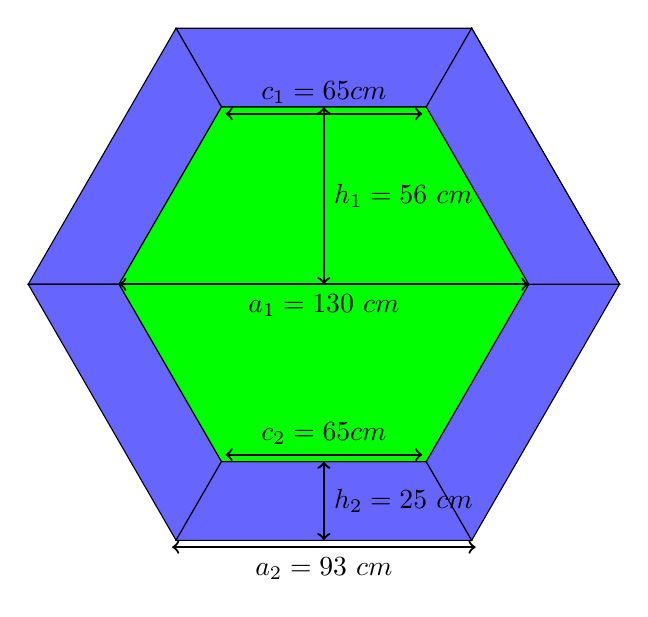
\begin{tikzpicture}
%Ich rechne mal sqrt(0.75) da hier ein gleichseitiges Dreieck vorliegt, bei dem man die Höhe berechnen muss.
%Dies geht mit dem Pythagoras, wobei der durch die Hälfte der Seite geht:
%               a²+b²=c² mit a=c/2 --> b²=c²-(c/2)²=c²-c²/4=3/4*c² --> b=c*sqrt(3/4)
%Flächenberechnung grün-blau in Python:
%R,h=50,25
%2*((2*R-R)*R*(0.75**0.5)/2)-6*((R+h*(0.75**0.5))-R)*h/2
  \pgfmathsetmacro{\hWert}{25}
  \pgfmathsetmacro{\RWert}{65}
  \pgfmathsetmacro{\dh}{\hWert/100*4}
  \pgfmathsetmacro{\R}{\RWert/100*4}
  \pgfmathsetmacro{\dR}{\dh/sqrt(0.75)}
  \pgfmathsetmacro{\hges}{(\R+\dR)*sqrt(0.75)}
  \pgfmathsetmacro{\h}{\hges-\dh}
%Schreibe ohne Komma
  \pgfmathtruncatemacro\gesamthoehe{2*(\RWert*sqrt(0.75)+\hWert)}
  \pgfmathtruncatemacro\aussenlaenge{\RWert+\hWert/sqrt(0.75)}
  \pgfmathtruncatemacro\innenlaenge{2*\RWert}
  \pgfmathtruncatemacro\innenhoehe{\RWert*sqrt(0.75)}
\foreach \rot in  {0,60,...,360}{
\draw[black,rotate=\rot,fill=blue!60] (\R,0) -- ++(\dR,0) -- ++(120:\R+\dR) -- ++(60:-\dR) -- cycle;
}
\draw[black,fill=green] (\R,0) -- ++(120:\R) -- ++(180:\R) -- ++(240:\R) -- ++(120:-\R) -- ++(0:\R) -- cycle ;
\draw[thick,<->] (-\R,0) --node[below] {$a_1=\innenlaenge~cm$} (\R,0);
\draw[thick,<->] (240:\R+\dR+0.1) --node[below] {$a_2=\aussenlaenge~cm$}  (300:\R+\dR+0.1);
\draw[thick,<->] (0,-\h) --node[right] {$h_2=\hWert~cm$} (0,-\hges);
\draw[thick,<->] (0,0) --node[right] {$h_1=\innenhoehe~cm$} (0,\h);
\draw[thick,<->] (240:\R-0.1) --node[above] {$c_2=\RWert cm$}  (300:\R-0.1);
\draw[thick,<->] (60:\R-0.1) --node[above] {$c_1=\RWert cm$}  (120:\R-0.1);
\end{tikzpicture}
$\begin{aligned}
geg.: a_1 &=130~cm& & \\
  c_1 &=65~cm& & \\
  h_1 &=162:2-25=56~cm& & \\
  a_2 &=93~cm& & \\
  c_2 &=65~cm& & \\
  h_2 &=25~cm & \\
ges.: A_{Gruen} &=?~cm^2& & \\
 A_{Blau} &=?~cm^2& & \\
& & & \\
A_{Gruen}&= 2\cdot (\frac12(a_1+c_1)\cdot h_1) & & \\
&= 2\cdot (\frac12(130+65)\cdot 56) & & \\
\makebox[0pt][l]{\uuline{\phantom{$A_{Gruen}=10.920~cm^2   \\$} } }
A_{Gruen}&=10.920~cm^2 & & \\
& & & \\
A_{blau}&= 6\cdot (\frac12(a_2+c_2)\cdot h_2) & & \\
&= 6\cdot (\frac12(93+65)\cdot 25) & & \\
\makebox[0pt][l]{\uuline{\phantom{$A_{blau}=11.915,06~cm^2   \\$} } }
A_{blau}&=11.915,06~cm^2 & & \\
\end{aligned}$
Die blaue Fläche ist größer.
}
\\\hline
g)&\pbox{7cm}{
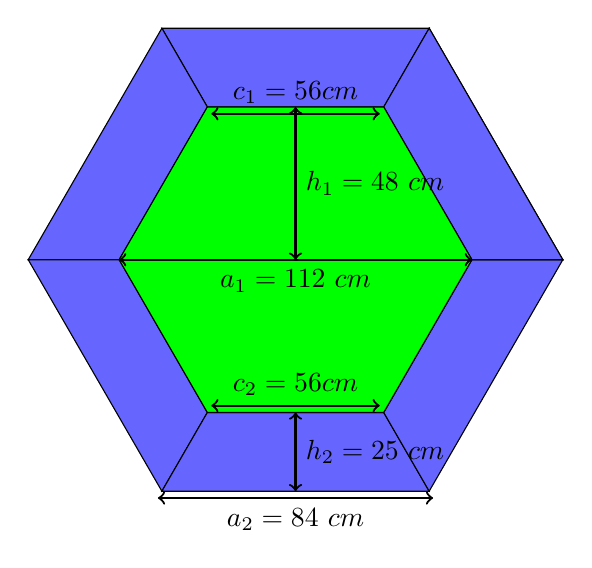
\begin{tikzpicture}
%Ich rechne mal sqrt(0.75) da hier ein gleichseitiges Dreieck vorliegt, bei dem man die Höhe berechnen muss.
%Dies geht mit dem Pythagoras, wobei der durch die Hälfte der Seite geht:
%               a²+b²=c² mit a=c/2 --> b²=c²-(c/2)²=c²-c²/4=3/4*c² --> b=c*sqrt(3/4)
%Flächenberechnung grün-blau in Python:
%R,h=50,25
%2*((2*R-R)*R*(0.75**0.5)/2)-6*((R+h*(0.75**0.5))-R)*h/2
  \pgfmathsetmacro{\hWert}{25}
  \pgfmathsetmacro{\RWert}{56}
  \pgfmathsetmacro{\dh}{\hWert/100*4}
  \pgfmathsetmacro{\R}{\RWert/100*4}
  \pgfmathsetmacro{\dR}{\dh/sqrt(0.75)}
  \pgfmathsetmacro{\hges}{(\R+\dR)*sqrt(0.75)}
  \pgfmathsetmacro{\h}{\hges-\dh}
%Schreibe ohne Komma
  \pgfmathtruncatemacro\gesamthoehe{2*(\RWert*sqrt(0.75)+\hWert)}
  \pgfmathtruncatemacro\aussenlaenge{\RWert+\hWert/sqrt(0.75)}
  \pgfmathtruncatemacro\innenlaenge{2*\RWert}
  \pgfmathtruncatemacro\innenhoehe{\RWert*sqrt(0.75)}
\foreach \rot in  {0,60,...,360}{
\draw[black,rotate=\rot,fill=blue!60] (\R,0) -- ++(\dR,0) -- ++(120:\R+\dR) -- ++(60:-\dR) -- cycle;
}
\draw[black,fill=green] (\R,0) -- ++(120:\R) -- ++(180:\R) -- ++(240:\R) -- ++(120:-\R) -- ++(0:\R) -- cycle ;
\draw[thick,<->] (-\R,0) --node[below] {$a_1=\innenlaenge~cm$} (\R,0);
\draw[thick,<->] (240:\R+\dR+0.1) --node[below] {$a_2=\aussenlaenge~cm$}  (300:\R+\dR+0.1);
\draw[thick,<->] (0,-\h) --node[right] {$h_2=\hWert~cm$} (0,-\hges);
\draw[thick,<->] (0,0) --node[right] {$h_1=\innenhoehe~cm$} (0,\h);
\draw[thick,<->] (240:\R-0.1) --node[above] {$c_2=\RWert cm$}  (300:\R-0.1);
\draw[thick,<->] (60:\R-0.1) --node[above] {$c_1=\RWert cm$}  (120:\R-0.1);
\end{tikzpicture}
$\begin{aligned}
geg.: a_1 &=112~cm& & \\
  c_1 &=56~cm& & \\
  h_1 &=146:2-25=48~cm& & \\
  a_2 &=84~cm& & \\
  c_2 &=56~cm& & \\
  h_2 &=25~cm & \\
ges.: A_{Gruen} &=?~cm^2& & \\
 A_{Blau} &=?~cm^2& & \\
& & & \\
A_{Gruen}&= 2\cdot (\frac12(a_1+c_1)\cdot h_1) & & \\
&= 2\cdot (\frac12(112+56)\cdot 48) & & \\
\makebox[0pt][l]{\uuline{\phantom{$A_{Gruen}=8.064~cm^2   \\$} } }
A_{Gruen}&=8.064~cm^2 & & \\
& & & \\
A_{blau}&= 6\cdot (\frac12(a_2+c_2)\cdot h_2) & & \\
&= 6\cdot (\frac12(84+56)\cdot 25) & & \\
\makebox[0pt][l]{\uuline{\phantom{$A_{blau}=10.565,06~cm^2   \\$} } }
A_{blau}&=10.565,06~cm^2 & & \\
\end{aligned}$
Die blaue Fläche ist größer.
}
\\\hline
h)&\pbox{7cm}{
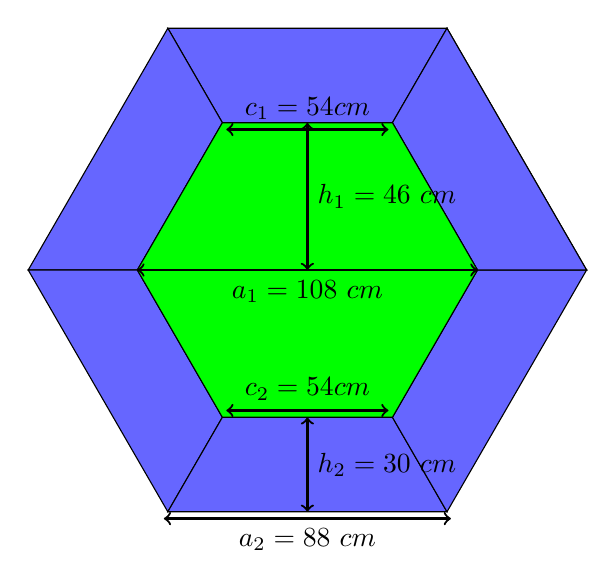
\begin{tikzpicture}
%Ich rechne mal sqrt(0.75) da hier ein gleichseitiges Dreieck vorliegt, bei dem man die Höhe berechnen muss.
%Dies geht mit dem Pythagoras, wobei der durch die Hälfte der Seite geht:
%               a²+b²=c² mit a=c/2 --> b²=c²-(c/2)²=c²-c²/4=3/4*c² --> b=c*sqrt(3/4)
%Flächenberechnung grün-blau in Python:
%R,h=50,25
%2*((2*R-R)*R*(0.75**0.5)/2)-6*((R+h*(0.75**0.5))-R)*h/2
  \pgfmathsetmacro{\hWert}{30}
  \pgfmathsetmacro{\RWert}{54}
  \pgfmathsetmacro{\dh}{\hWert/100*4}
  \pgfmathsetmacro{\R}{\RWert/100*4}
  \pgfmathsetmacro{\dR}{\dh/sqrt(0.75)}
  \pgfmathsetmacro{\hges}{(\R+\dR)*sqrt(0.75)}
  \pgfmathsetmacro{\h}{\hges-\dh}
%Schreibe ohne Komma
  \pgfmathtruncatemacro\gesamthoehe{2*(\RWert*sqrt(0.75)+\hWert)}
  \pgfmathtruncatemacro\aussenlaenge{\RWert+\hWert/sqrt(0.75)}
  \pgfmathtruncatemacro\innenlaenge{2*\RWert}
  \pgfmathtruncatemacro\innenhoehe{\RWert*sqrt(0.75)}
\foreach \rot in  {0,60,...,360}{
\draw[black,rotate=\rot,fill=blue!60] (\R,0) -- ++(\dR,0) -- ++(120:\R+\dR) -- ++(60:-\dR) -- cycle;
}
\draw[black,fill=green] (\R,0) -- ++(120:\R) -- ++(180:\R) -- ++(240:\R) -- ++(120:-\R) -- ++(0:\R) -- cycle ;
\draw[thick,<->] (-\R,0) --node[below] {$a_1=\innenlaenge~cm$} (\R,0);
\draw[thick,<->] (240:\R+\dR+0.1) --node[below] {$a_2=\aussenlaenge~cm$}  (300:\R+\dR+0.1);
\draw[thick,<->] (0,-\h) --node[right] {$h_2=\hWert~cm$} (0,-\hges);
\draw[thick,<->] (0,0) --node[right] {$h_1=\innenhoehe~cm$} (0,\h);
\draw[thick,<->] (240:\R-0.1) --node[above] {$c_2=\RWert cm$}  (300:\R-0.1);
\draw[thick,<->] (60:\R-0.1) --node[above] {$c_1=\RWert cm$}  (120:\R-0.1);
\end{tikzpicture}
$\begin{aligned}
geg.: a_1 &=108~cm& & \\
  c_1 &=54~cm& & \\
  h_1 &=152:2-30=46~cm& & \\
  a_2 &=88~cm& & \\
  c_2 &=54~cm& & \\
  h_2 &=30~cm & \\
ges.: A_{Gruen} &=?~cm^2& & \\
 A_{Blau} &=?~cm^2& & \\
& & & \\
A_{Gruen}&= 2\cdot (\frac12(a_1+c_1)\cdot h_1) & & \\
&= 2\cdot (\frac12(108+54)\cdot 46) & & \\
\makebox[0pt][l]{\uuline{\phantom{$A_{Gruen}=7.452~cm^2   \\$} } }
A_{Gruen}&=7.452~cm^2 & & \\
& & & \\
A_{blau}&= 6\cdot (\frac12(a_2+c_2)\cdot h_2) & & \\
&= 6\cdot (\frac12(88+54)\cdot 30) & & \\
\makebox[0pt][l]{\uuline{\phantom{$A_{blau}=12.837,69~cm^2   \\$} } }
A_{blau}&=12.837,69~cm^2 & & \\
\end{aligned}$
Die blaue Fläche ist größer.
}
\\\hline
\end{xltabular}
\vspace{0.5cm}
\end{document}